\section{Πειραματική Αξιολόγηση}
\subsection{Μελέτη εντολών άλματος}
Στο παρόν τμήμα της εργασίας συλλέγουμε στατιστικά για το είδος εντολών άλματος των benchmarks που θα εκτελέσουμε.

\vspace{3mm}
   \begin{minipage}{\textwidth}
      \begin{center}
         \fbox{\textlatin{\textbf{\textit{403-gcc}}}}\\
         \vspace{3mm}
         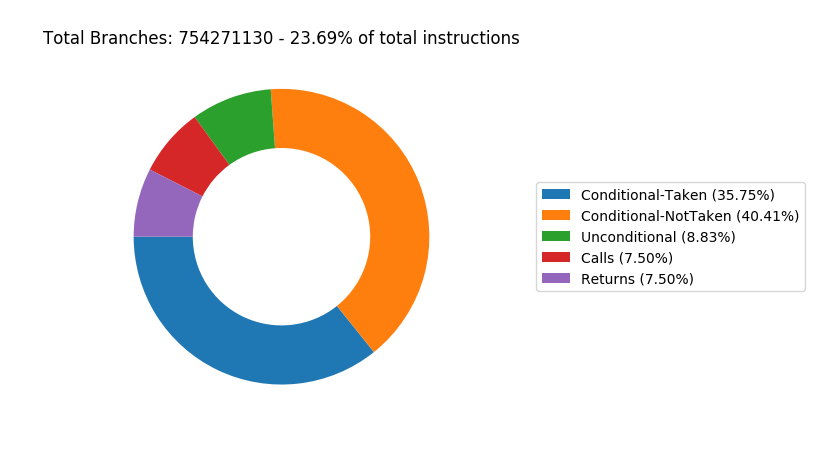
\includegraphics[width=0.9\textwidth, frame]{./graphs/4-1/403-gcc.png}
         \vspace{6mm}
      \end{center}
   \end{minipage}

   \begin{minipage}{\textwidth}
      \begin{center}
         \fbox{\textlatin{\textbf{\textit{429-mcf}}}}\\
         \vspace{3mm}
         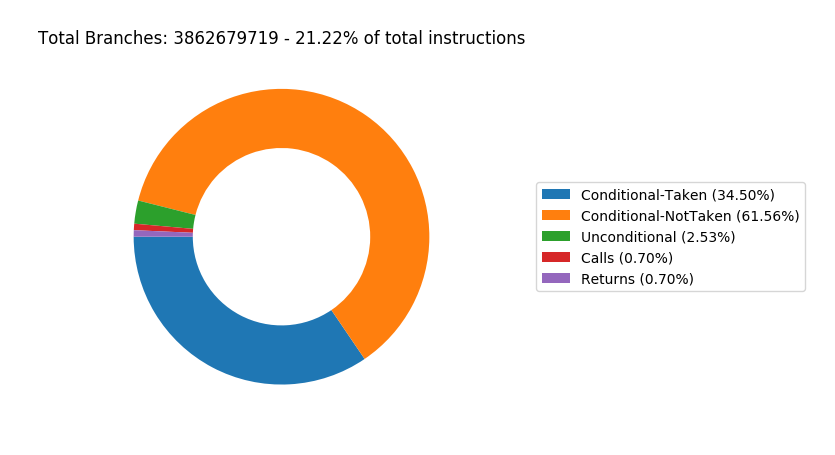
\includegraphics[width=0.9\textwidth, frame]{./graphs/4-1/429-mcf.png}
         \vspace{6mm}
      \end{center}
   \end{minipage}

   \begin{minipage}{\textwidth}
      \begin{center}
         \fbox{\textlatin{\textbf{\textit{434-zeusmp}}}}\\
         \vspace{3mm}
         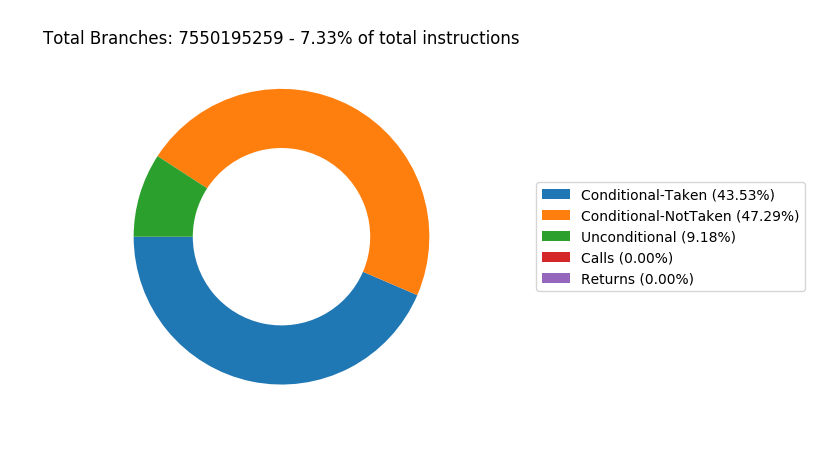
\includegraphics[width=0.9\textwidth, frame]{./graphs/4-1/434-zeusmp.png}
         \vspace{6mm}
      \end{center}
   \end{minipage}

   \begin{minipage}{\textwidth}
      \begin{center}
         \fbox{\textlatin{\textbf{\textit{436-cactusADM}}}}\\
         \vspace{3mm}
         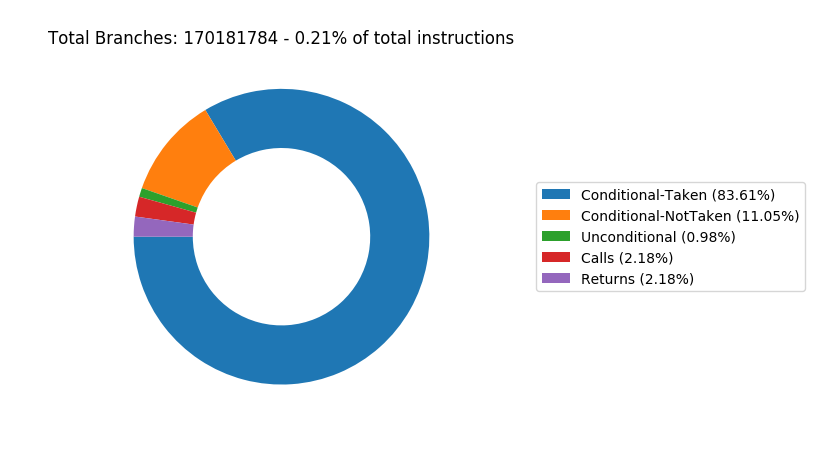
\includegraphics[width=0.9\textwidth, frame]{./graphs/4-1/436-cactusADM.png}
         \vspace{6mm}
      \end{center}
   \end{minipage}

   \begin{minipage}{\textwidth}
      \begin{center}
         \fbox{\textlatin{\textbf{\textit{445-gobmk}}}}\\
         \vspace{3mm}
         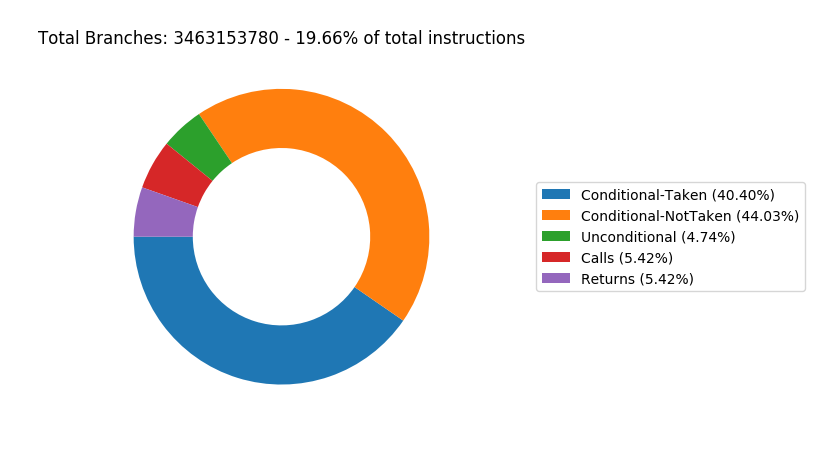
\includegraphics[width=0.9\textwidth, frame]{./graphs/4-1/445-gobmk.png}
         \vspace{6mm}
      \end{center}
   \end{minipage}

   \begin{minipage}{\textwidth}
      \begin{center}
         \fbox{\textlatin{\textbf{\textit{450-soplex}}}}\\
         \vspace{3mm}
         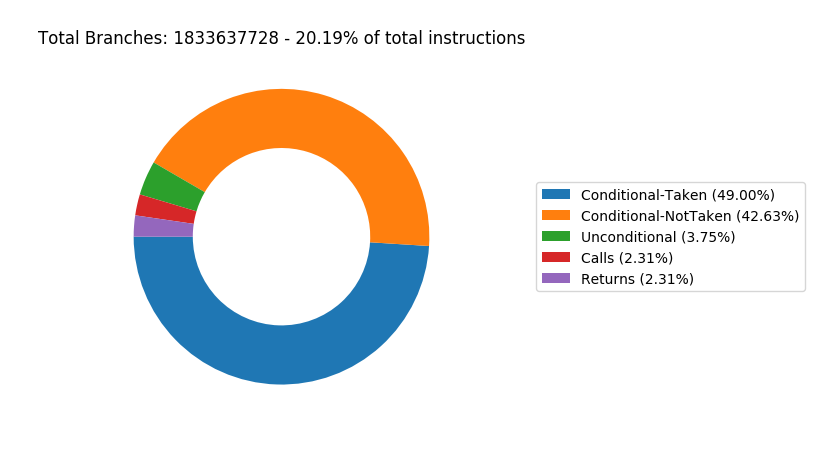
\includegraphics[width=0.9\textwidth, frame]{./graphs/4-1/450-soplex.png}
         \vspace{6mm}
      \end{center}
   \end{minipage}

   \begin{minipage}{\textwidth}
      \begin{center}
         \fbox{\textlatin{\textbf{\textit{456-hmmer}}}}\\
         \vspace{3mm}
         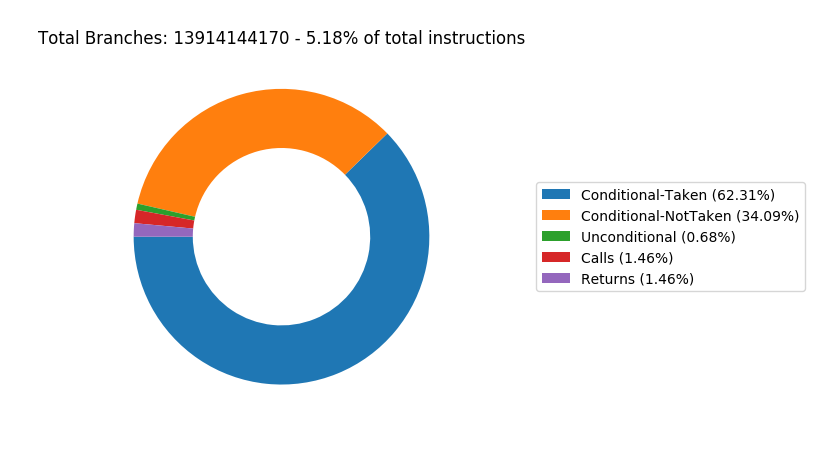
\includegraphics[width=0.9\textwidth, frame]{./graphs/4-1/456-hmmer.png}
         \vspace{6mm}
      \end{center}
   \end{minipage}

   \begin{minipage}{\textwidth}
      \begin{center}
         \fbox{\textlatin{\textbf{\textit{458-sjeng}}}}\\
         \vspace{3mm}
         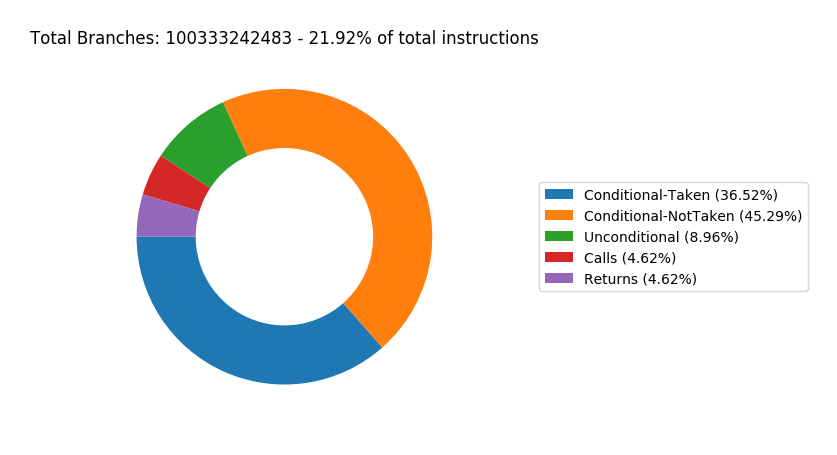
\includegraphics[width=0.9\textwidth, frame]{./graphs/4-1/458-sjeng.png}
         \vspace{6mm}
      \end{center}
   \end{minipage}

   \begin{minipage}{\textwidth}
      \begin{center}
         \fbox{\textlatin{\textbf{\textit{459-GemsFDTD}}}}\\
         \vspace{3mm}
         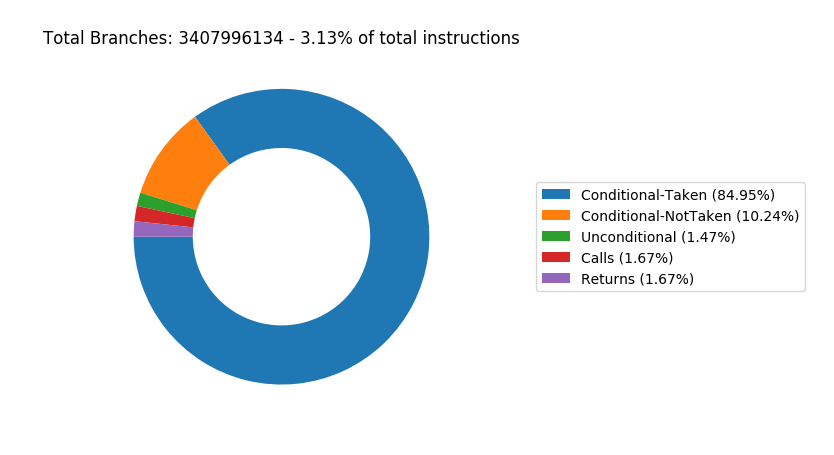
\includegraphics[width=0.9\textwidth, frame]{./graphs/4-1/459-GemsFDTD.png}
         \vspace{6mm}
      \end{center}
   \end{minipage}

   \begin{minipage}{\textwidth}
      \begin{center}
         \fbox{\textlatin{\textbf{\textit{471-omnetpp}}}}\\
         \vspace{3mm}
         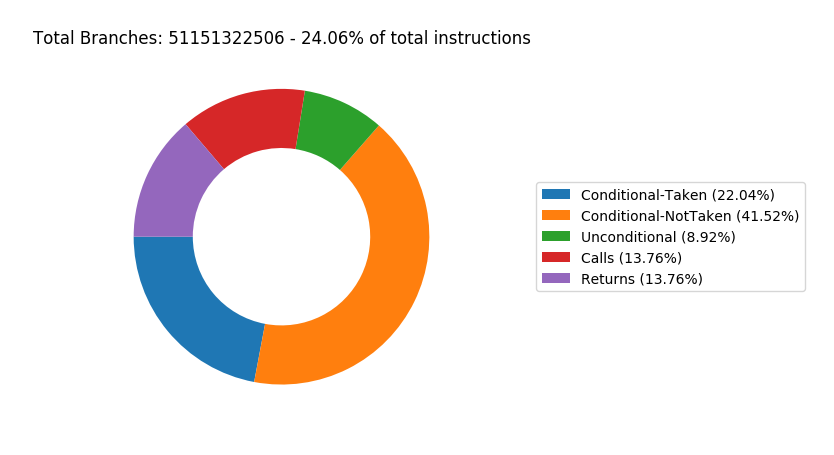
\includegraphics[width=0.9\textwidth, frame]{./graphs/4-1/471-omnetpp.png}
         \vspace{6mm}
      \end{center}
   \end{minipage}

   \begin{minipage}{\textwidth}
      \begin{center}
         \fbox{\textlatin{\textbf{\textit{473-astar}}}}\\
         \vspace{3mm}
         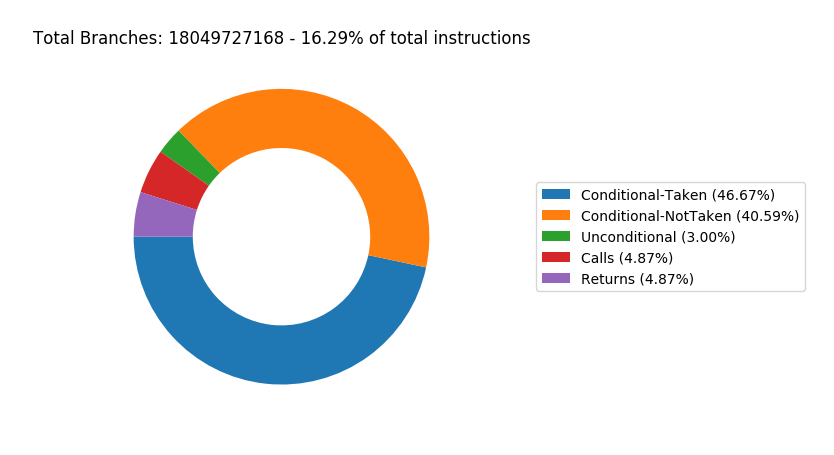
\includegraphics[width=0.9\textwidth, frame]{./graphs/4-1/473-astar.png}
         \vspace{6mm}
      \end{center}
   \end{minipage}

   \begin{minipage}{\textwidth}
      \begin{center}
         \fbox{\textlatin{\textbf{\textit{483-xalancbmk}}}}\\
         \vspace{3mm}
         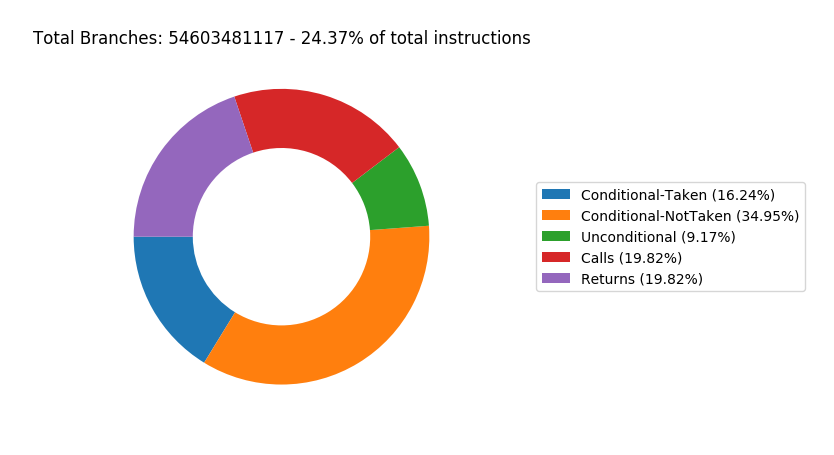
\includegraphics[width=0.9\textwidth, frame]{./graphs/4-1/483-xalancbmk.png}
         \vspace{6mm}
      \end{center}
   \end{minipage}

   \begin{minipage}{\textwidth}
      \begin{center}
         \vspace{3mm}
         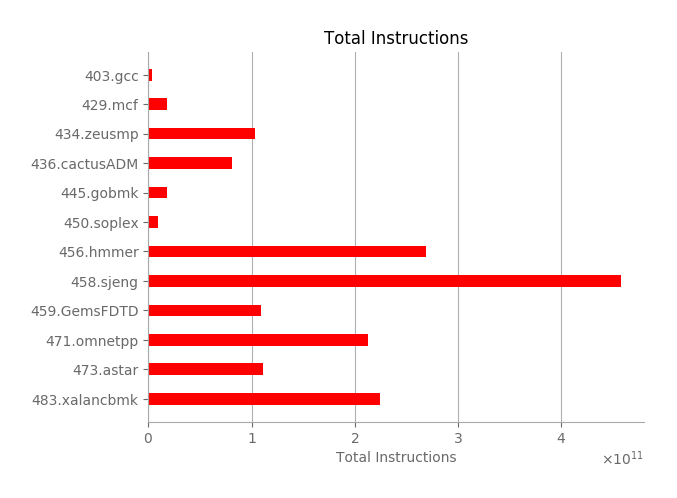
\includegraphics[width=0.8\textwidth, frame]{./graphs/4-1/total.png}
         \vspace{6mm}
      \end{center}
   \end{minipage}

   \paragraph{Σχόλια}\vspace{1em}

   Από τα παραπάνω διαγράμματα παρατηρούμε ότι στα μετροπρογράμματά μας οι
   εντολές άλματος αποτελούν ένα σημαντικό ποσοστό των συνολικών εντολών που
   εκτελούνται. Υπάρχουν benchmarks όπου οι εντολές άλματος είναι περίπου το
   20\%-30\% των συνολικών εντολών (403.gcc, 429.mcf, 445.gobmk, 450.soplex,
   458.sjeng, 483.xalancbmk, 473.astar) και άλλα όπου οι εντολές άλματος είναι
   σημαντικά λιγότερες κάτω του 5\% των συνολικών (459.GemsFDTD και
   436.cactusADM).
   
   Οσον αφορά την κατηγορία των αλμάτων, τα περισσότερα από αυτά τα είναι είτε
   Conditional Taken, είτε Conditional NotTaken. Αρκετά λιγότερα (συνολικά περί
   το 10\%) είναι τα Unconditional Branches, Calls, Returns.
   
   Τέλος, για το σύνολο των εντολών, όπως βλέπουμε στο σψετικό ραβδόγραμμα,
   υπάρχουν benchmarks με μικρό πλήθος εντολών (gcc, mcf, zeusmp, soplex, gobmk)
   και άλλα με αρκετά μεγάλο πλήθος εντολών τα οποία απαιτούν και μεγαλύτερο
   χρόνο εκτέλεσης (hmmer, sjeng, omnetop).
   